% !TeX document-id = {143f66d8-ef22-4f31-8276-701c8691dfde}
% Copyright 2007 by Till Tantau
%
% This file may be distributed and/or modified
%
% 1. under the LaTeX Project Public License and/or
% 2. under the GNU Public License.
%
% See the file doc/licenses/LICENSE for more details.



\documentclass{beamer}
%use only for handouts
%\usepackage{handoutWithNotes}
%\pgfpagesuselayout{4 on 1 with notes}[a4paper,border shrink=5mm]
% Setup appearance:

\usepackage{xcolor}								% Colorful headings
\definecolor{LutraGreen}{RGB}{19,170,72} 
\definecolor{LutraGrey}{RGB}{80,80,80} 

\usetheme{lutra}
\usefonttheme[onlylarge]{structurebold}
\setbeamerfont*{frametitle}{size=\normalsize,series=\bfseries}
\setbeamertemplate{navigation symbols}{}
\setbeamercolor{block title}{bg=white,fg=LutraGreen}
\setbeamercolor*{item}{fg=LutraGreen}
\setbeamercolor{section in toc}{fg=LutraGreen}

% Standard packages

\usepackage[english]{babel}
\usepackage[latin1]{inputenc}
%\usepackage{times}
\usepackage{multimedia} 
\usepackage{media9}
\usepackage[T1]{fontenc}
%\usepackage[sfdefault]{roboto}

\usepackage{hyperref}


% Setup TikZ

\usepackage{tikz}
\usetikzlibrary{arrows}
\tikzstyle{block}=[draw opacity=0.7,line width=1.4cm]

% Author, Title, etc.

\title{QGIS LTR is making the world a better place}

\author{Saber Razmjooei}

\date{6 October 2015}


\begin{document}

% The main document


\begin{frame}
  \titlepage
\end{frame}

\begin{frame}[allowframebreaks]{Outline}
  \setcounter{tocdepth}{2}
  \tableofcontents
\end{frame}


\section{Understanding release cycle}
\AtBeginSection[]
{
	\begin{frame}<beamer>
		\frametitle{Plan}
		\tableofcontents[currentsection]
	\end{frame}
}
\subsection{Current releases}
\begin{frame}{Why so many versions?}
	\centering{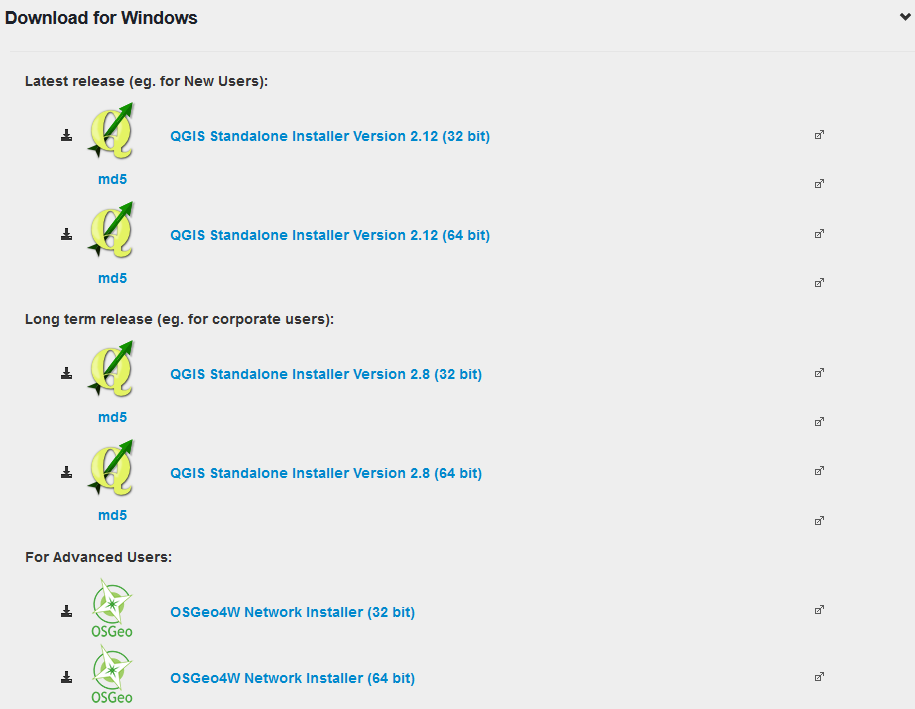
\includegraphics[width=0.8\textwidth]{windows_download.png}}
\end{frame}

\begin{frame}{Keeping everyone happy}
	\centering{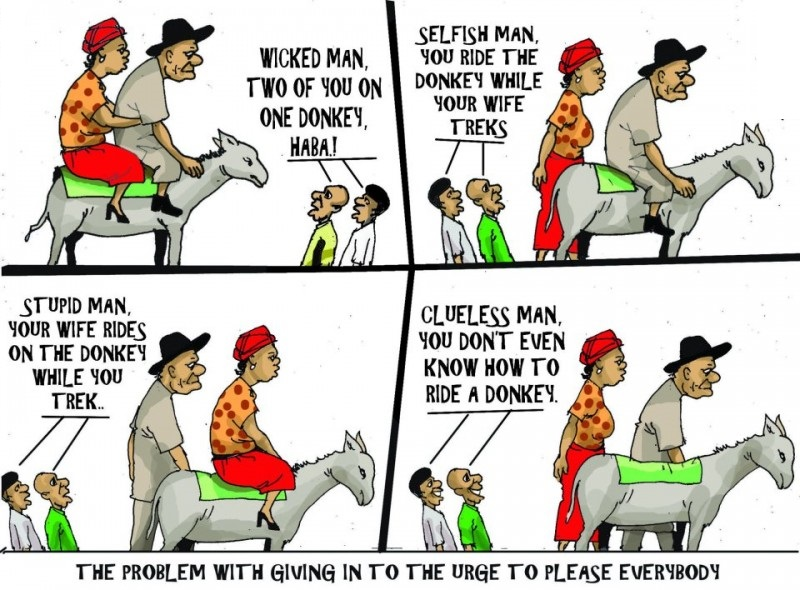
\includegraphics[width=0.8\textwidth]{You-can-not-please-everyone.jpg}}
\end{frame}

\begin{frame}{Versions}
	\begin{block}{QGIS versions}
		\begin{itemize}
			\item Development or nightly (DEV)
			\item Release (LR) 
			\item Long Term Release (LTR)
		\end{itemize}
	\end{block}
\end{frame}

\begin{frame}{QGIS release - LTR, LR, DEV}
	\centering{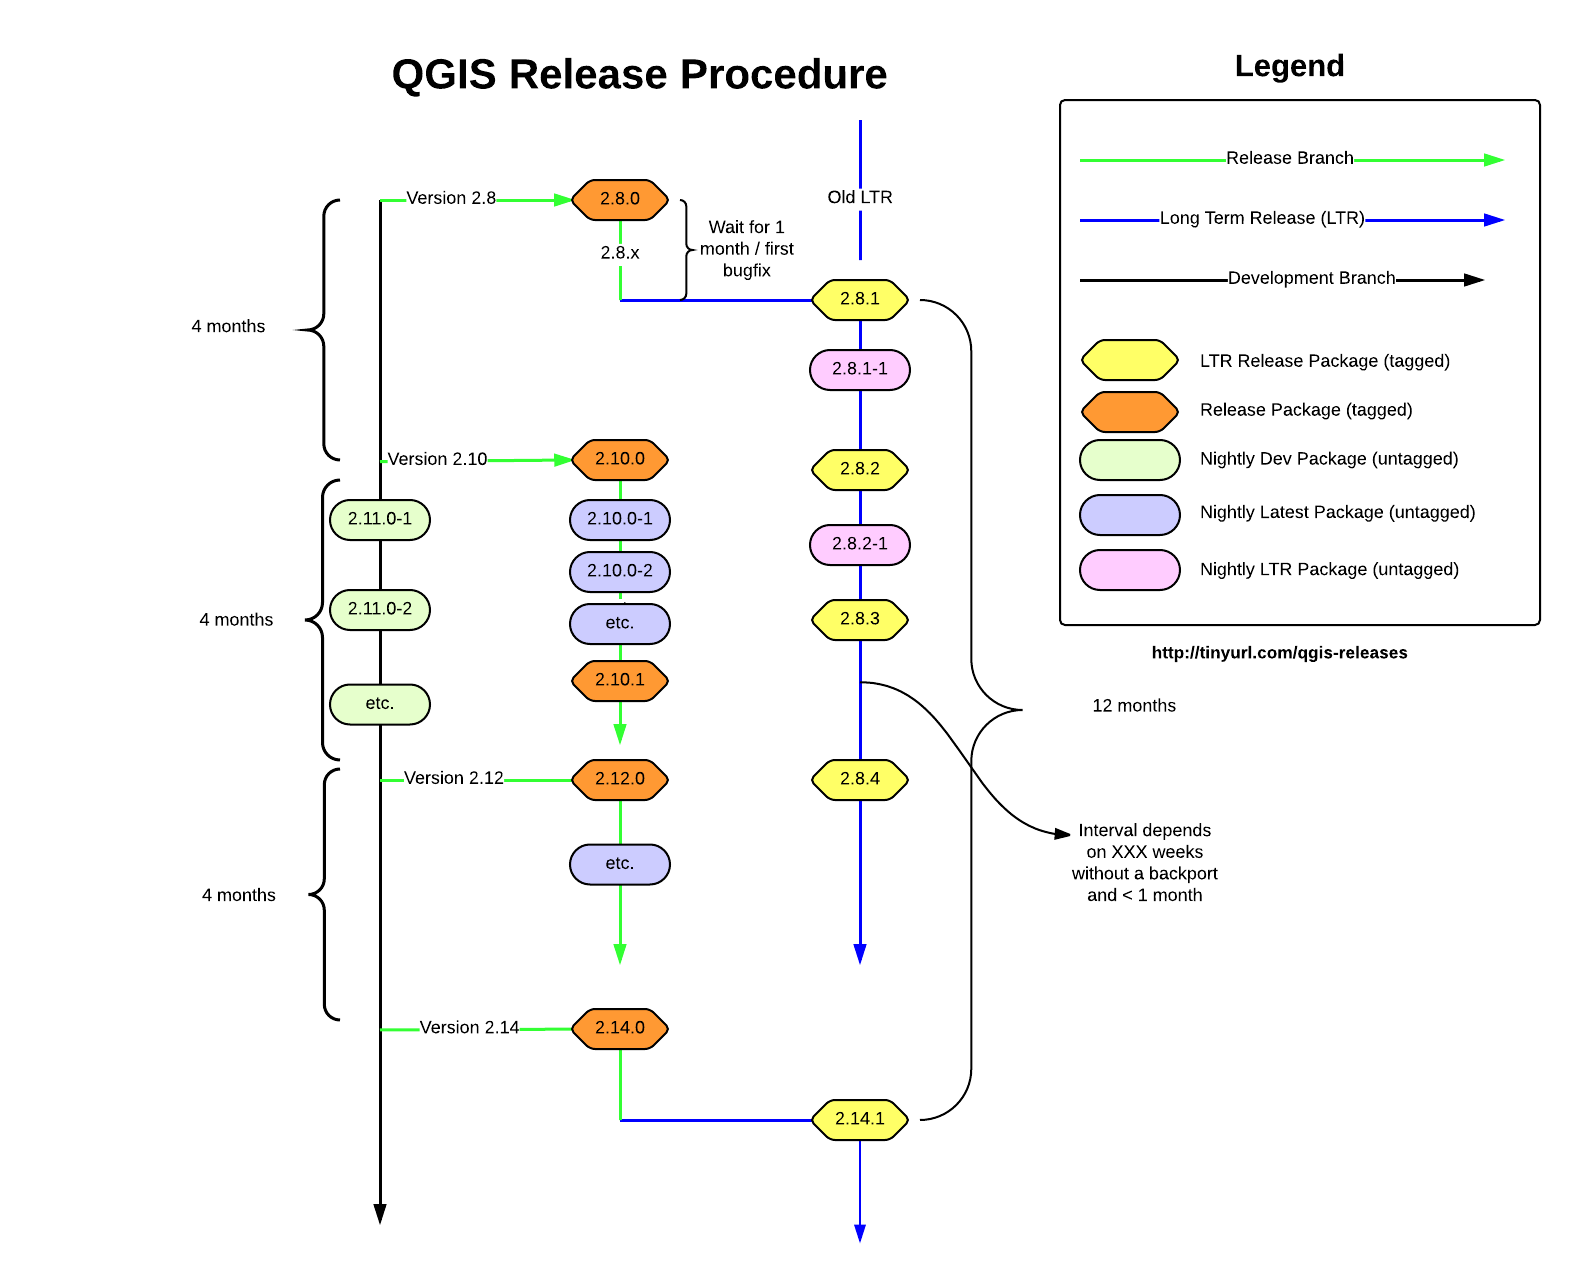
\includegraphics[width=0.9\textwidth]{ae1c0956-523e-11e4-95d9-cea1a3429faf.png}}
\end{frame}

\begin{frame}{Development version}
	\begin{block}{Suitable for:}
		\begin{itemize}
			\item Core developers
			\item Plugin developers
			\item Curious about bleeding edge features!
		\end{itemize}
	\end{block}
\end{frame}

\begin{frame}{Release version}
	\begin{block}{Suitable for:}
		\begin{itemize}
			\item New users
			\item If you want new features without burning down your house!
		\end{itemize}
	\end{block}
\end{frame}

\subsection{LTR}
\begin{frame}{LTR version}
	\begin{block}{Suitable for:}
		\begin{itemize}
			\item Corporate users
		\end{itemize}
	\end{block}
\end{frame}

\begin{frame}{LTR}
	\begin{block}{What is LTR?}
		\begin{itemize}
			\item Supported period
			\item Software bugs 
			\item No new features
			\item Release cycle
		\end{itemize}
	\end{block}
\end{frame}

\begin{frame}{LTR}
	\begin{block}{Why LTR?}
		\begin{itemize}
			\item Reliability
			\item Stability
			\item Less frequent release cycle 
		\end{itemize}
	\end{block}
\end{frame}

\begin{frame}{LTR}
	\begin{block}{2.8 in numbers}
		\begin{itemize}
			\item 4 releases: 2.8.0, 2.8.1, 2.8.2 and 2.8.3
			\item 184 bugs closed
			\item 630 commits on github since 2.7 feature freeze:
			\begin{itemize}
				\item 2.8.0: 325
				\item 2.8.1: +33
				\item 2.8.2: +122
				\item 2.8.3: +150
			\end{itemize}
			\item 758734 downloads\footnote{Windows stand-alone installer only}
			\begin{itemize}
				\item 2.8.0: 324
				\item 2.8.1: 363474
				\item 2.8.2: 306721
				\item 2.8.3: 88215
			\end{itemize}			
		\end{itemize}
	\end{block}
\end{frame}

\begin{frame}{LTR}
	\begin{block}{Why NOT LTR?}
		\begin{itemize}
			\item Users
				\begin{itemize}
					\item New features
				\end{itemize}		
			\item Developers 
				\begin{itemize}
					\item Extra cost
					\item Extra resources
					\item Adding features is more fun!
				\end{itemize}
		\end{itemize}
	\end{block}
\end{frame}

\subsection{2.x releases}
\begin{frame}{QGIS 2.x releases}
	\begin{block}{Release early, release often}
		\begin{itemize}
			\item 3 moths of development
			\item 1 month of bug fix
		\end{itemize}
	\end{block}
	\begin{center}

	\begin{tabular}{|c|c|}
		\hline QGIS release & Date \\ 
		\hline 2.0\footnote{To coincide with FOSS4G in Nottingham} & September 2013 \\ 
		\hline 2.2 & February 2014 \\ 
		\hline 2.4 & June 2014 \\ 
		\hline 2.6\footnote{Delayed by a week} & November 2014 \\ 
		\hline {\color{red}\textbf{2.8}} & {\color{red}\textbf{February 2015}} \\ 
		\hline 2.10 & June 2015 \\ 
		\hline 2.12 & October 2015 \\ 
		\hline {\color{red} \textit{2.14}} & {\color{red}\textit{February 2016}} \\ 
		\hline 
	\end{tabular} 
	\end{center} 
\end{frame}


\subsection{Past problems}
\begin{frame}{QGIS release - problems}
	\begin{block}{Less reliable software:}
		\begin{itemize}
			\item Bug reporting participation
			\item Planned releasing 
			\item Regressions and blockers
		\end{itemize}
	\end{block}
	\begin{center}
		
		\begin{tabular}{|c|c|}
			\hline QGIS release & No. of bugs closed \\ 
			\hline 2.0\footnote{Change of API} & 1075 \\ 
			\hline 2.2 & 71 \\ 
			\hline 2.4 & 191 \\ 
			\hline 2.6 & 100 \\ 
			\hline 2.8\footnote{Sum of 2.8.x releases} & 184 \\ 
			\hline 
		\end{tabular}
	\end{center} 
\end{frame}


\section{How to support QGIS (LTR)?}

\begin{frame}{How to support QGIS (LTR)?}
	\begin{block}{You can:}
		\begin{itemize}
			\item Sponsor bug fixing
				\begin{itemize}
					\item Donation to QGIS
					\item Contracting QGIS developer(s)
				\end{itemize}
		\end{itemize}
	\end{block}
	
	\begin{center}
		\begin{tabular}{|c|c|}
			\hline Sponsorship & Amount \euro \\ 
			\hline Platinum Sponsor & 27,000 + \\ 
			\hline Gold Sponsor & 9,000 +  \\ 
			\hline Silver Sponsor & 3,000 + \\ 
			\hline Bronze Sponsor & 500 + \\ 
			\hline 
		\end{tabular}
	\end{center}
	
	http://qgis.org/en/site/getinvolved/donations.html
\end{frame}

\begin{frame}{How to support QGIS (LTR)?}
	\centering{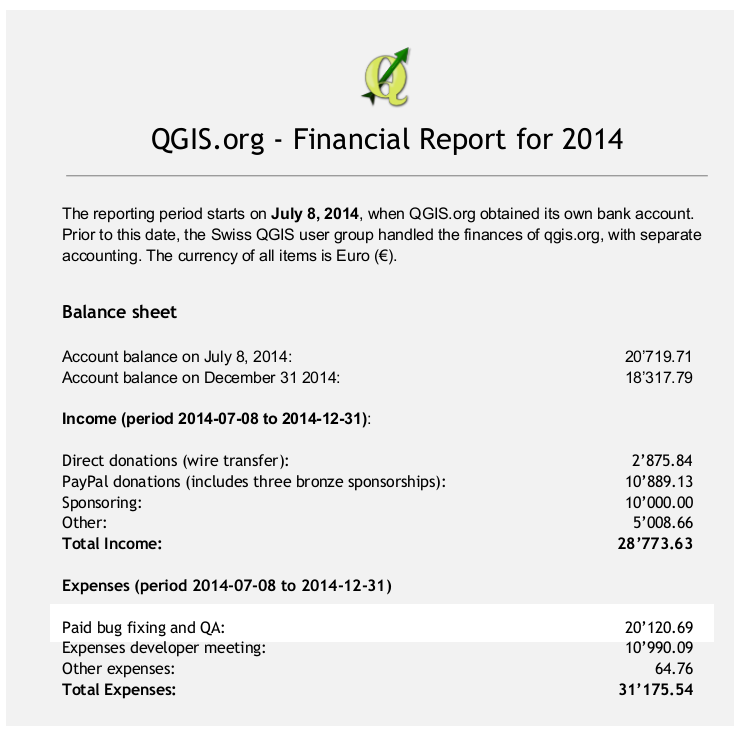
\includegraphics[width=0.7\textwidth]{PublicQGISfinancialreport2014.png}}
\end{frame}

\begin{frame}{How to support QGIS (LTR)?}
	\centering{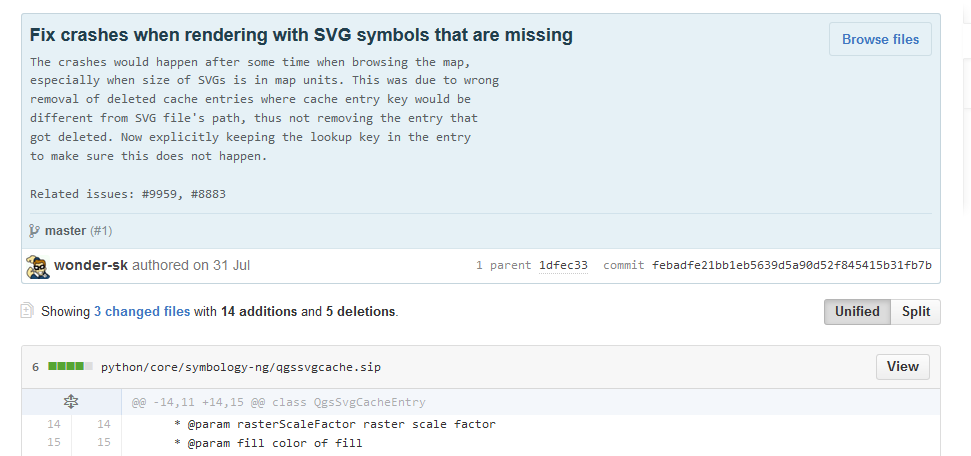
\includegraphics[width=0.8\textwidth]{svg-fix.png}}
\end{frame}

\begin{frame}{How to support QGIS (LTR)?}
	\begin{block}{You can:}
		\begin{itemize}
			\item Participate
			\begin{itemize}
				\item Testing
				\begin{itemize}
					\item Run multiple QGIS versions
					\item Test previous bugs
					\item Try new features
					\item Help with other reported bugs
				\end{itemize}
				\item Filing bugs (https://hub.qgis.org/projects/quantum-gis/issues):
				\begin{itemize}
					\item Step-by-step guide to reproduce your bug
					\item Follow-ups
					\item Provide test data
				\end{itemize}
			\end{itemize}
		\end{itemize}
	\end{block}
\end{frame}

\section{Future plans}
\subsection{2.14 release}

\begin{frame}{Future plans}
	\begin{block}{QGIS 2.14 release}
		\begin{itemize}
			\item Preparing the code base for QGIS 3.0
			\item Bug fixing 
			\item Some new features
		\end{itemize}
	\end{block}
\end{frame}

\subsection{3.0 release}
\begin{frame}{Future plans}
	\begin{block}{QGIS 3.0}
		\begin{itemize}
			\item Support for QT5
			\item Upgrade to Python 3
			\item Change of API
		\end{itemize}
	\end{block}
\end{frame}

\subsection{Full-time developer}
\begin{frame}{Future plans}
	\begin{block}{Full time QGIS developer}
		\begin{itemize}
			\item Raising \pounds100k
		\end{itemize}
	\end{block}
\end{frame}

\section{QGIS Survey}

\begin{frame}{QGIS survey results}
	\begin{block}{User proficiency}
	\end{block}
	\centering{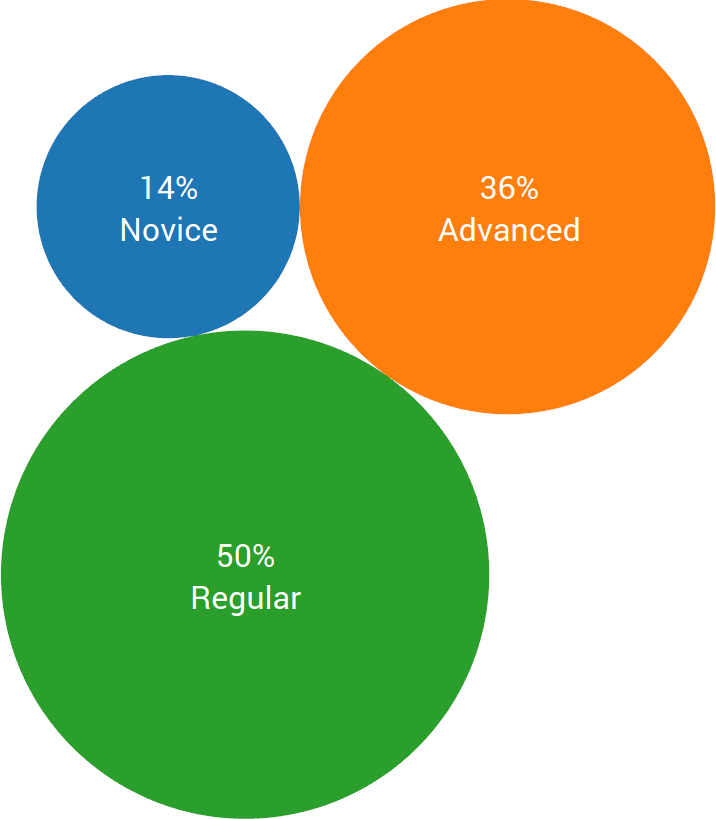
\includegraphics[width=0.4\textwidth]{qgis_survey_oct2015_1.png}}
\end{frame}

\begin{frame}{QGIS survey results}
	\begin{block}{Frequency of use}
	\end{block}
	\centering{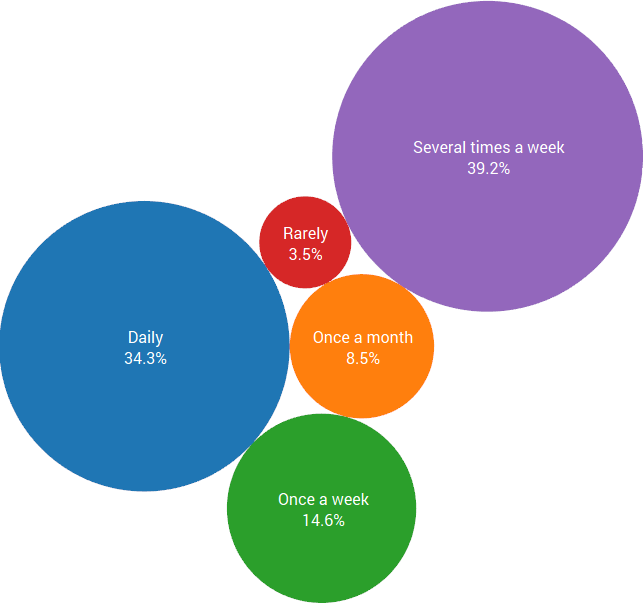
\includegraphics[width=0.6\textwidth]{qgis_survey_oct2015_2.png}}
\end{frame}

\begin{frame}{QGIS survey results}
	\begin{block}{Which version}
	\end{block}
	\centering{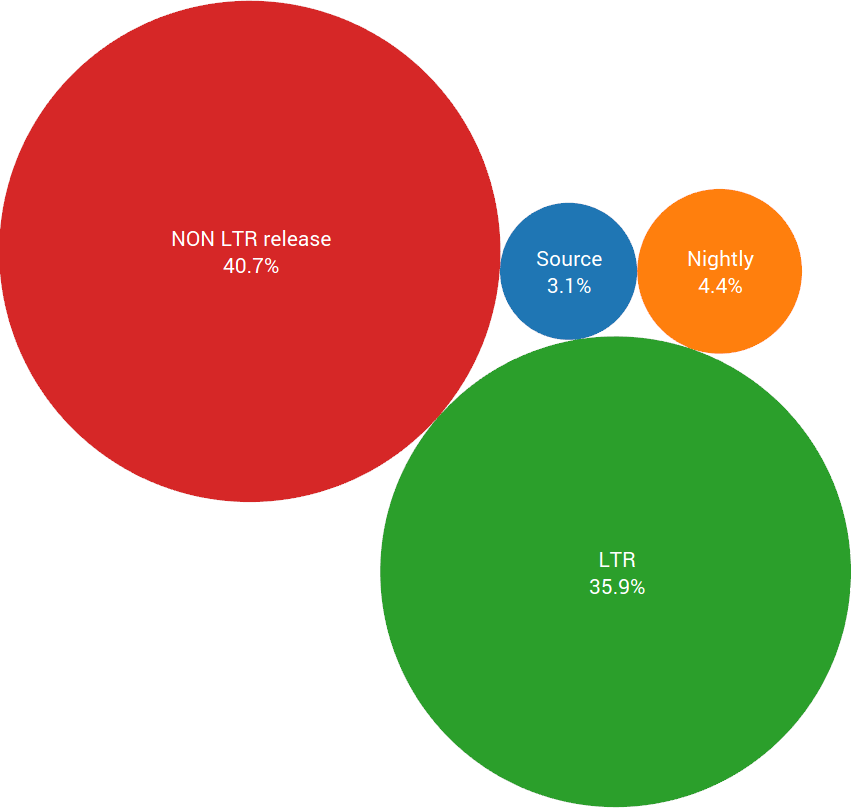
\includegraphics[width=0.6\textwidth]{qgis_survey_oct2015_3.png}}
\end{frame}

\begin{frame}{QGIS survey results}
	\begin{block}{Support period for the LTR}
	\end{block}
	\centering{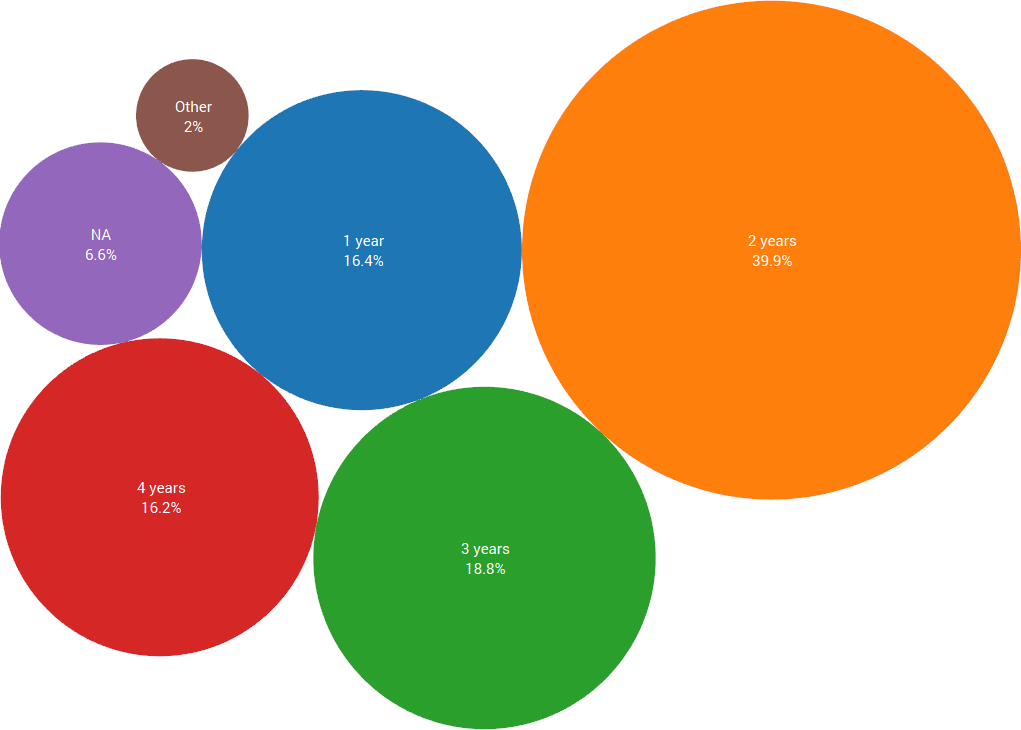
\includegraphics[width=0.85\textwidth]{qgis_survey_oct2015_4.png}}
\end{frame}

\begin{frame}{QGIS survey results}
	\begin{block}{Supporting QGIS project}
	\end{block}
	\centering{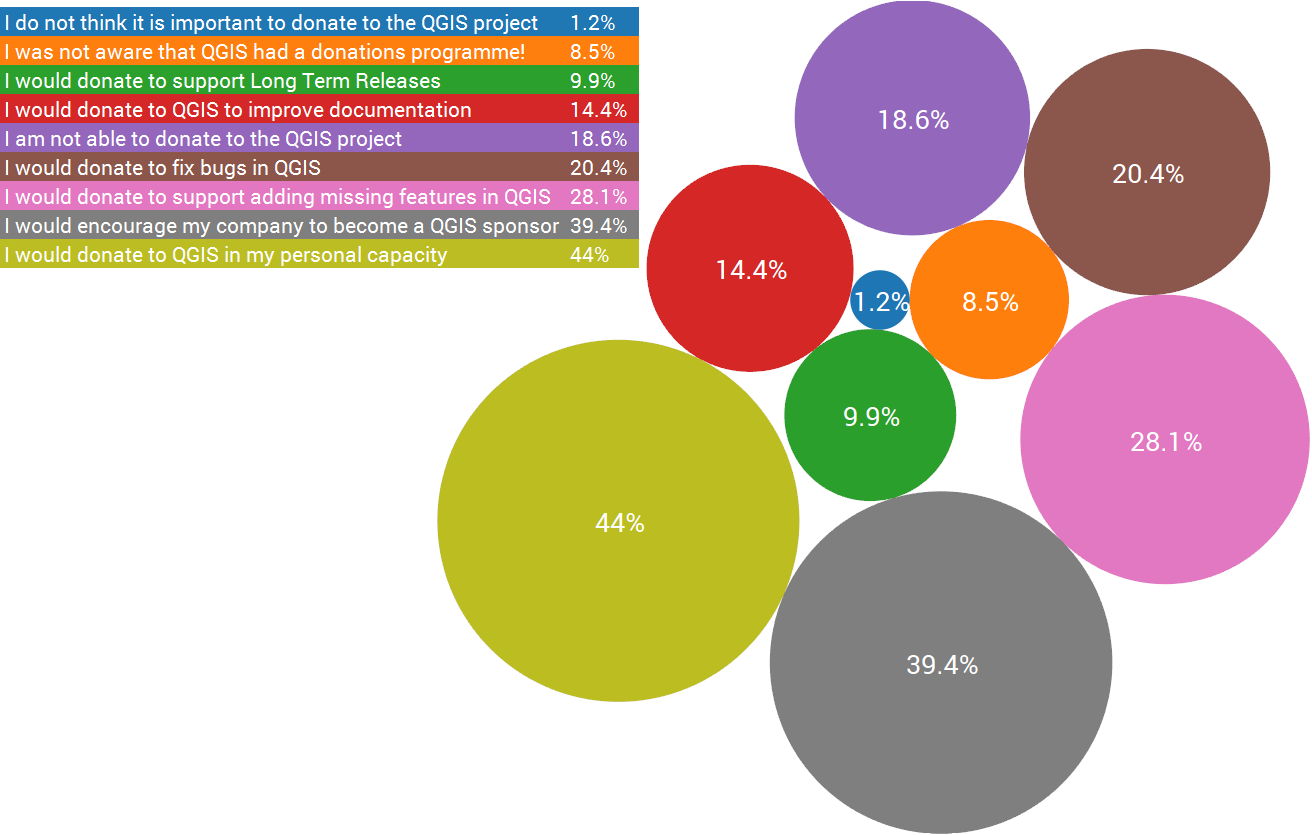
\includegraphics[width=0.95\textwidth]{qgis_survey_oct2015_5.png}}
\end{frame}

\begin{frame}{QGIS survey results}
	\begin{block}{Allocation of QGIS budget}
	\end{block}
	\centering{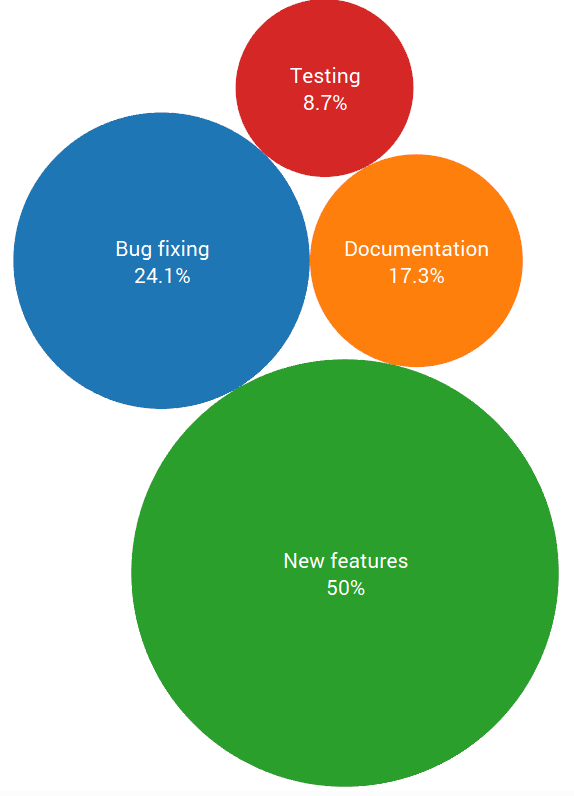
\includegraphics[width=0.45\textwidth]{qgis_survey_oct2015_6.png}}
\end{frame}

\section{New features in QGIS 2.12}
\begin{frame}{QGIS 2.12 - New features}
	\begin{block}{Label engine enhancement}
		\begin{itemize}
			\item Rule-based labelling
			\item Better positioning of labels
			\item Advanced displaying options
			\item Prioritisation of labels
		\end{itemize}
	\end{block}
\end{frame}

\begin{frame}{QGIS 2.12 - New features}
	\begin{block}{Analysis}
		\begin{itemize}
			\item Raster alignment tool
			\item Geometry checker
		\end{itemize}
	\end{block}
\end{frame}

\begin{frame}{QGIS 2.12 - New features}
	\begin{block}{Other major improvements}
		\begin{itemize}
			\item GRASS integration
			\item Map composer
			\item Encrypted passrwod management
			\item Mutually exclusive layer for groups in layer tree
			\item See full list here:http://www.qgis.org/en/site/forusers/visualchangelog212/
		\end{itemize}
	\end{block}
\end{frame}

\section{Case study}
\begin{frame}{QGIS LTR: Case study}
	\begin{block}{Custom installer}
		\begin{itemize}
			\item Pre-configured with data/services
			\item Includes templates (print composers, styles, etc.)
			\item Directly compiled from LTR source on github
			\item Plugin configuration
			\item GUI configuration
		\end{itemize}
	\end{block}
	\centering{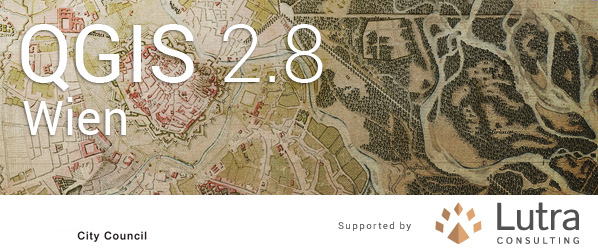
\includegraphics[width=0.7\textwidth]{b77ada24-3f76-11e5-808f-6686696e19f0.jpg}}
\end{frame}



\end{document}